
\newcommand{\figureKonzole}{
\begin{figure}[H]
    \centering
    
\includegraphics[width=8cm]{cs/obrazky/konzole.png}
    \caption{Konzole}
    \label{fig:konzole}
\end{figure}
}
\newcommand{\figureUkoly}{
\begin{figure}[H]
    \centering
    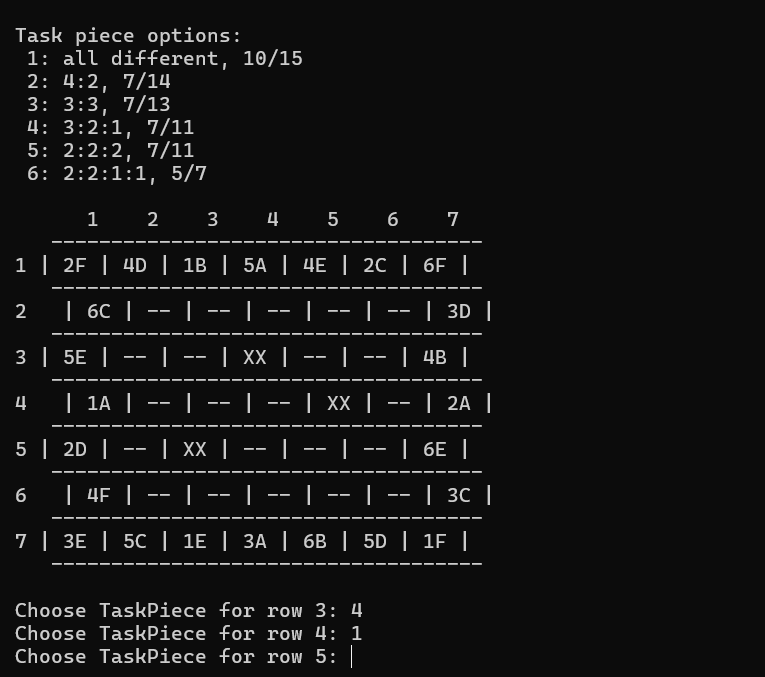
\includegraphics[width=8cm]{cs/obrazky/ukoly.png}
    \caption{Výběr úkolů na herní desku}
    \label{fig:ukoly}
\end{figure}
}
\newcommand{\figureSinglePlay}{
\begin{figure}[H]
    \centering
    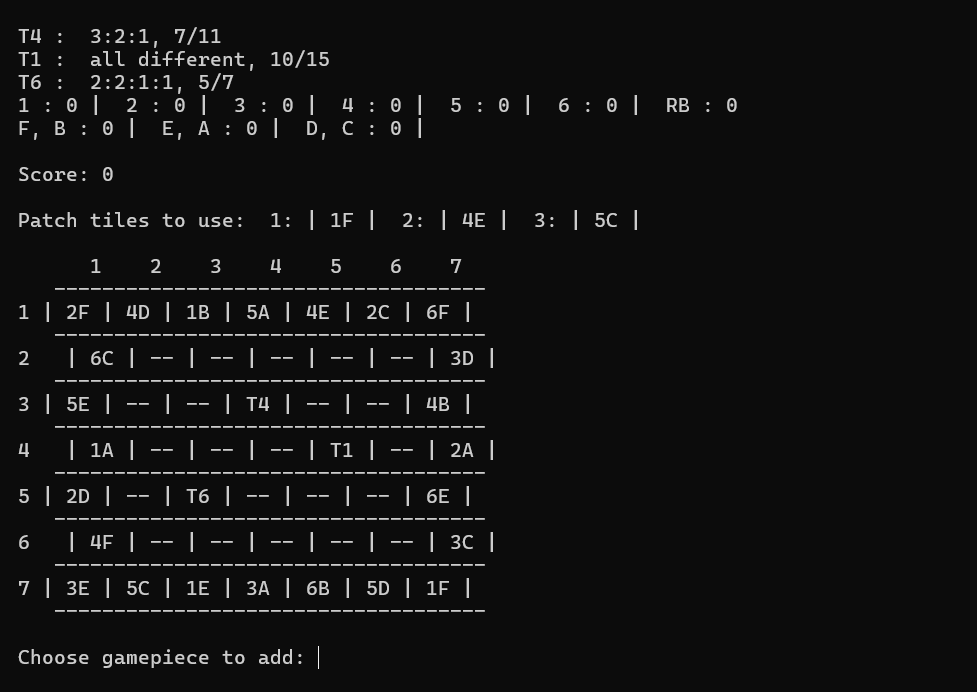
\includegraphics[width=8cm]{cs/obrazky/single.png}
    \caption{Stav hry pro jednoho hráče}
    \label{fig:singlePlay}
\end{figure}
}
\newcommand{\figureMultiPlay}{
\begin{figure}[H]
    \centering
    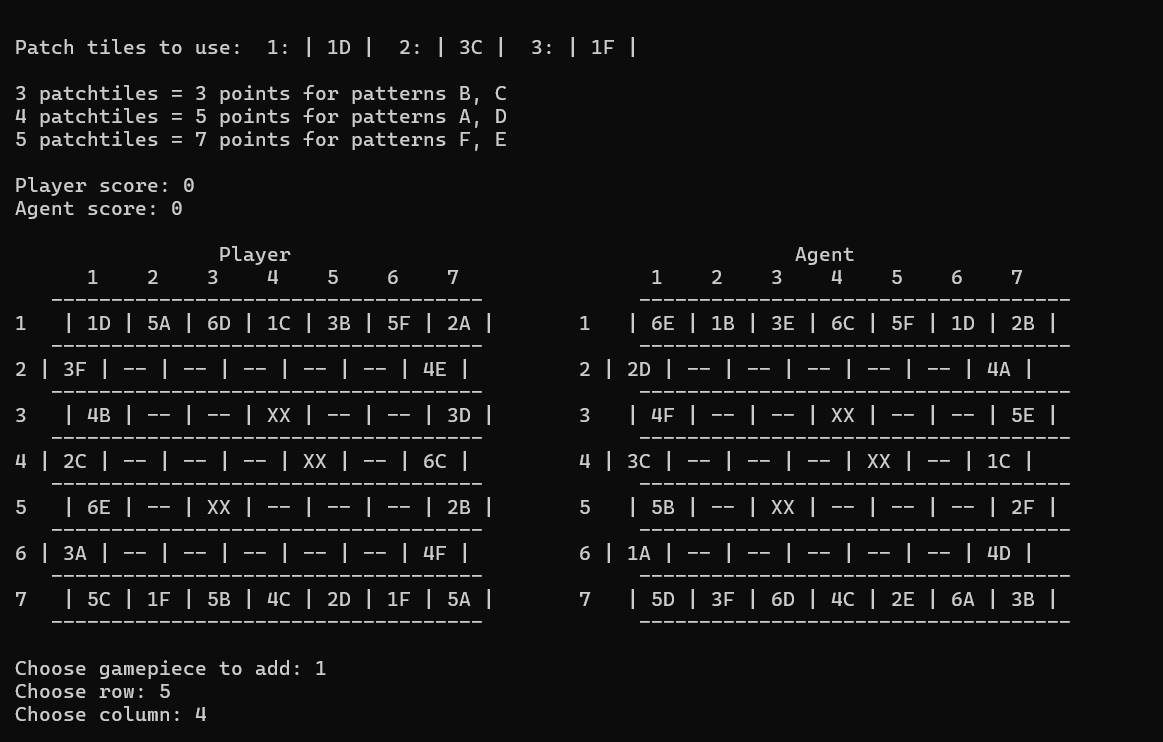
\includegraphics[width=8cm]{cs/obrazky/multi.png}
    \caption{Stav hry hráče proti počítači}
    \label{fig:multiPlay}
\end{figure}
}


\newcommand{\figureOmezeniHladovehoPristupuPriklad}{
\begin{figure}[H]
    \centering
    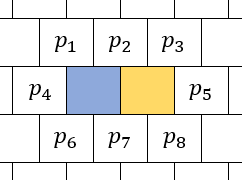
\includegraphics{cs/obrazky/stromoveProhledavaniPriklad.png}
    \caption{Příklad situace hry zjednodušené pouze na barvy dílků}
    \label{fig:omezeniHladovehoPristupuPriklad}
\end{figure}
}
\newcommand{\figureStrom}{
\begin{figure}[H]
    \centering
    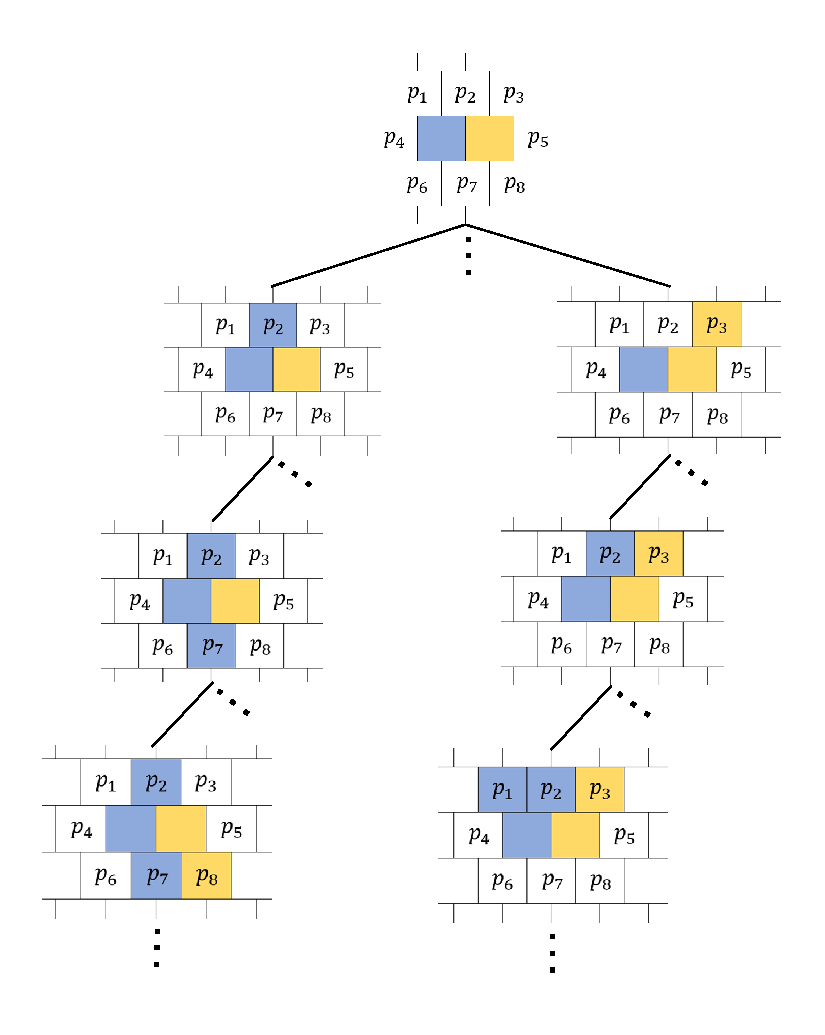
\includegraphics[width=10cm]{cs/obrazky/strom.pdf}
    \caption{Stromová reprezentace stavového prostoru}
    \label{fig:strom}
\end{figure}
}

\newcommand{\figureTS}{
\begin{figure}[H]
    \centering
    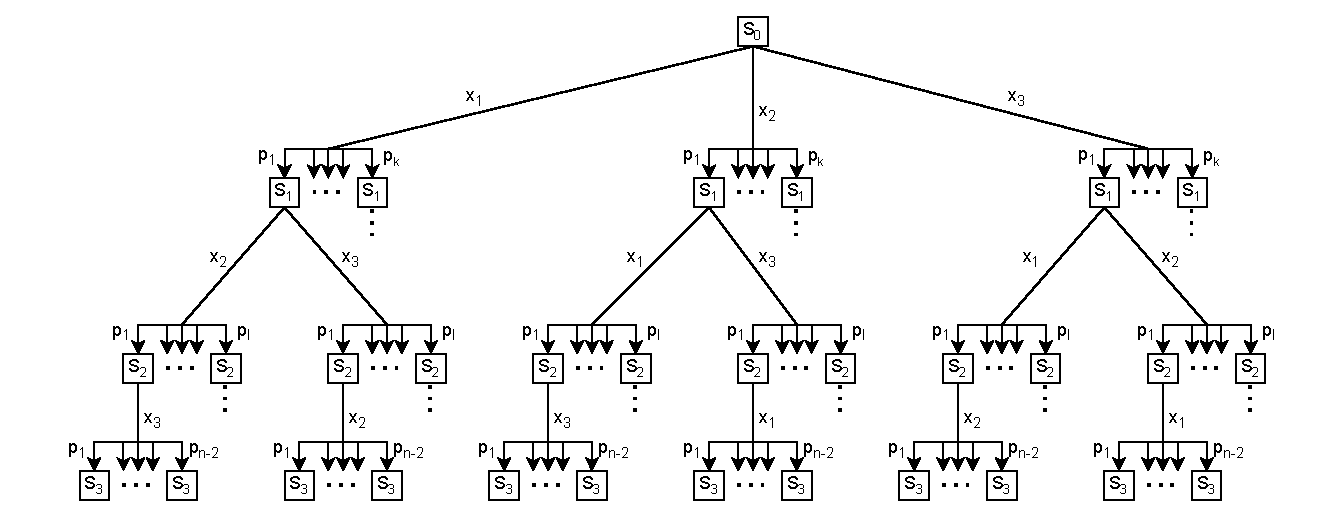
\includegraphics[width=14.7cm]{cs/obrazky/TS.pdf}
    \caption{Stromové prohledávání}
    \label{fig:TS}
\end{figure}
}

\newcommand{\figureMCTS}{
\begin{figure}[H]
    \centering
    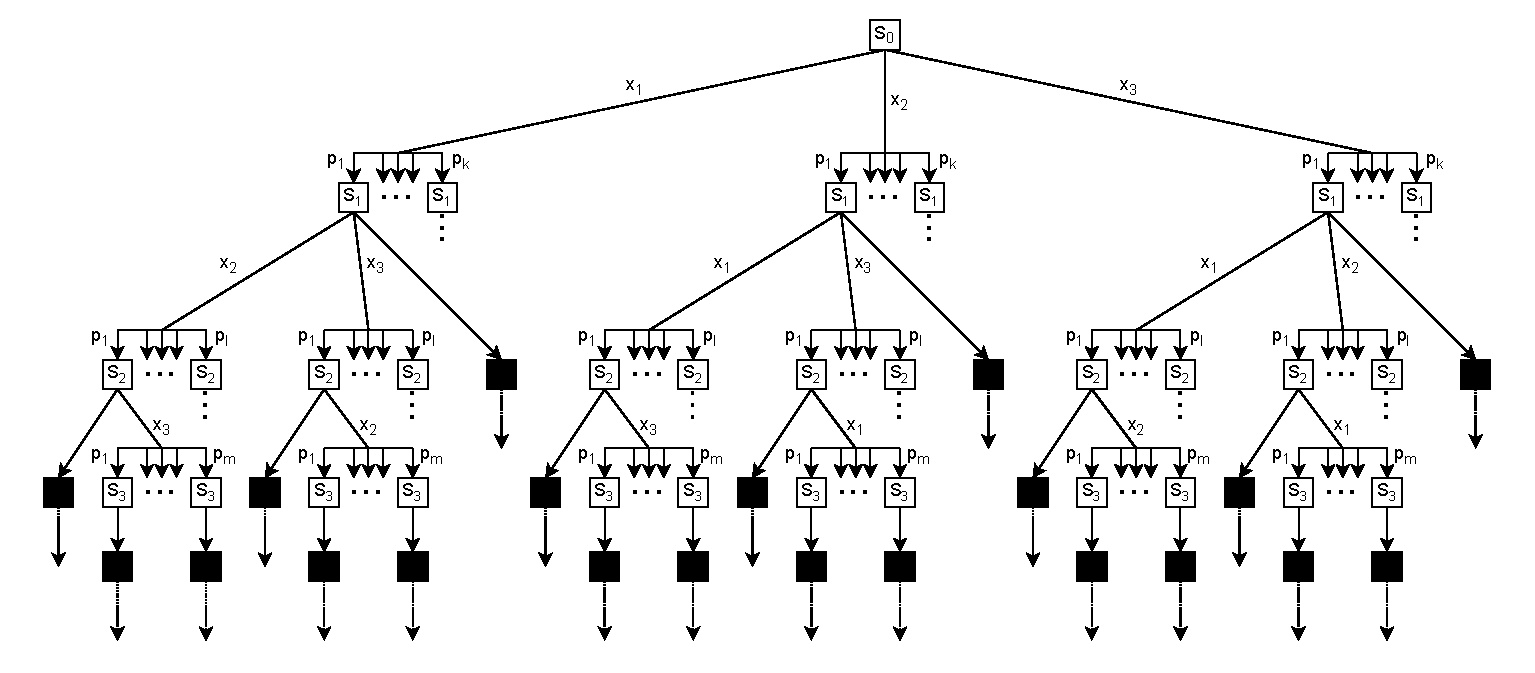
\includegraphics[width=14.7cm]{cs/obrazky/mc_tree.pdf}
    \caption{Stromové prohledávání inspirované MCTS}
    \label{fig:MCTS}
\end{figure}
}

\newcommand{\figureHerniDeska}{
\begin{figure}[H]
    \centering
    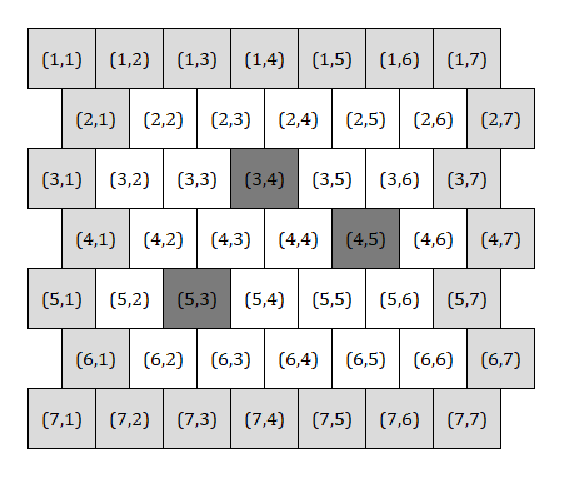
\includegraphics[width=7cm]{cs/obrazky/herniDeska.pdf}
    \caption{Reprezentace herní desky dvourozměrným polem}
    \label{fig:herniDeska}
\end{figure}
}

\newcommand{\figureZlepseniGraf}{
\begin{figure}[H]
    \centering
    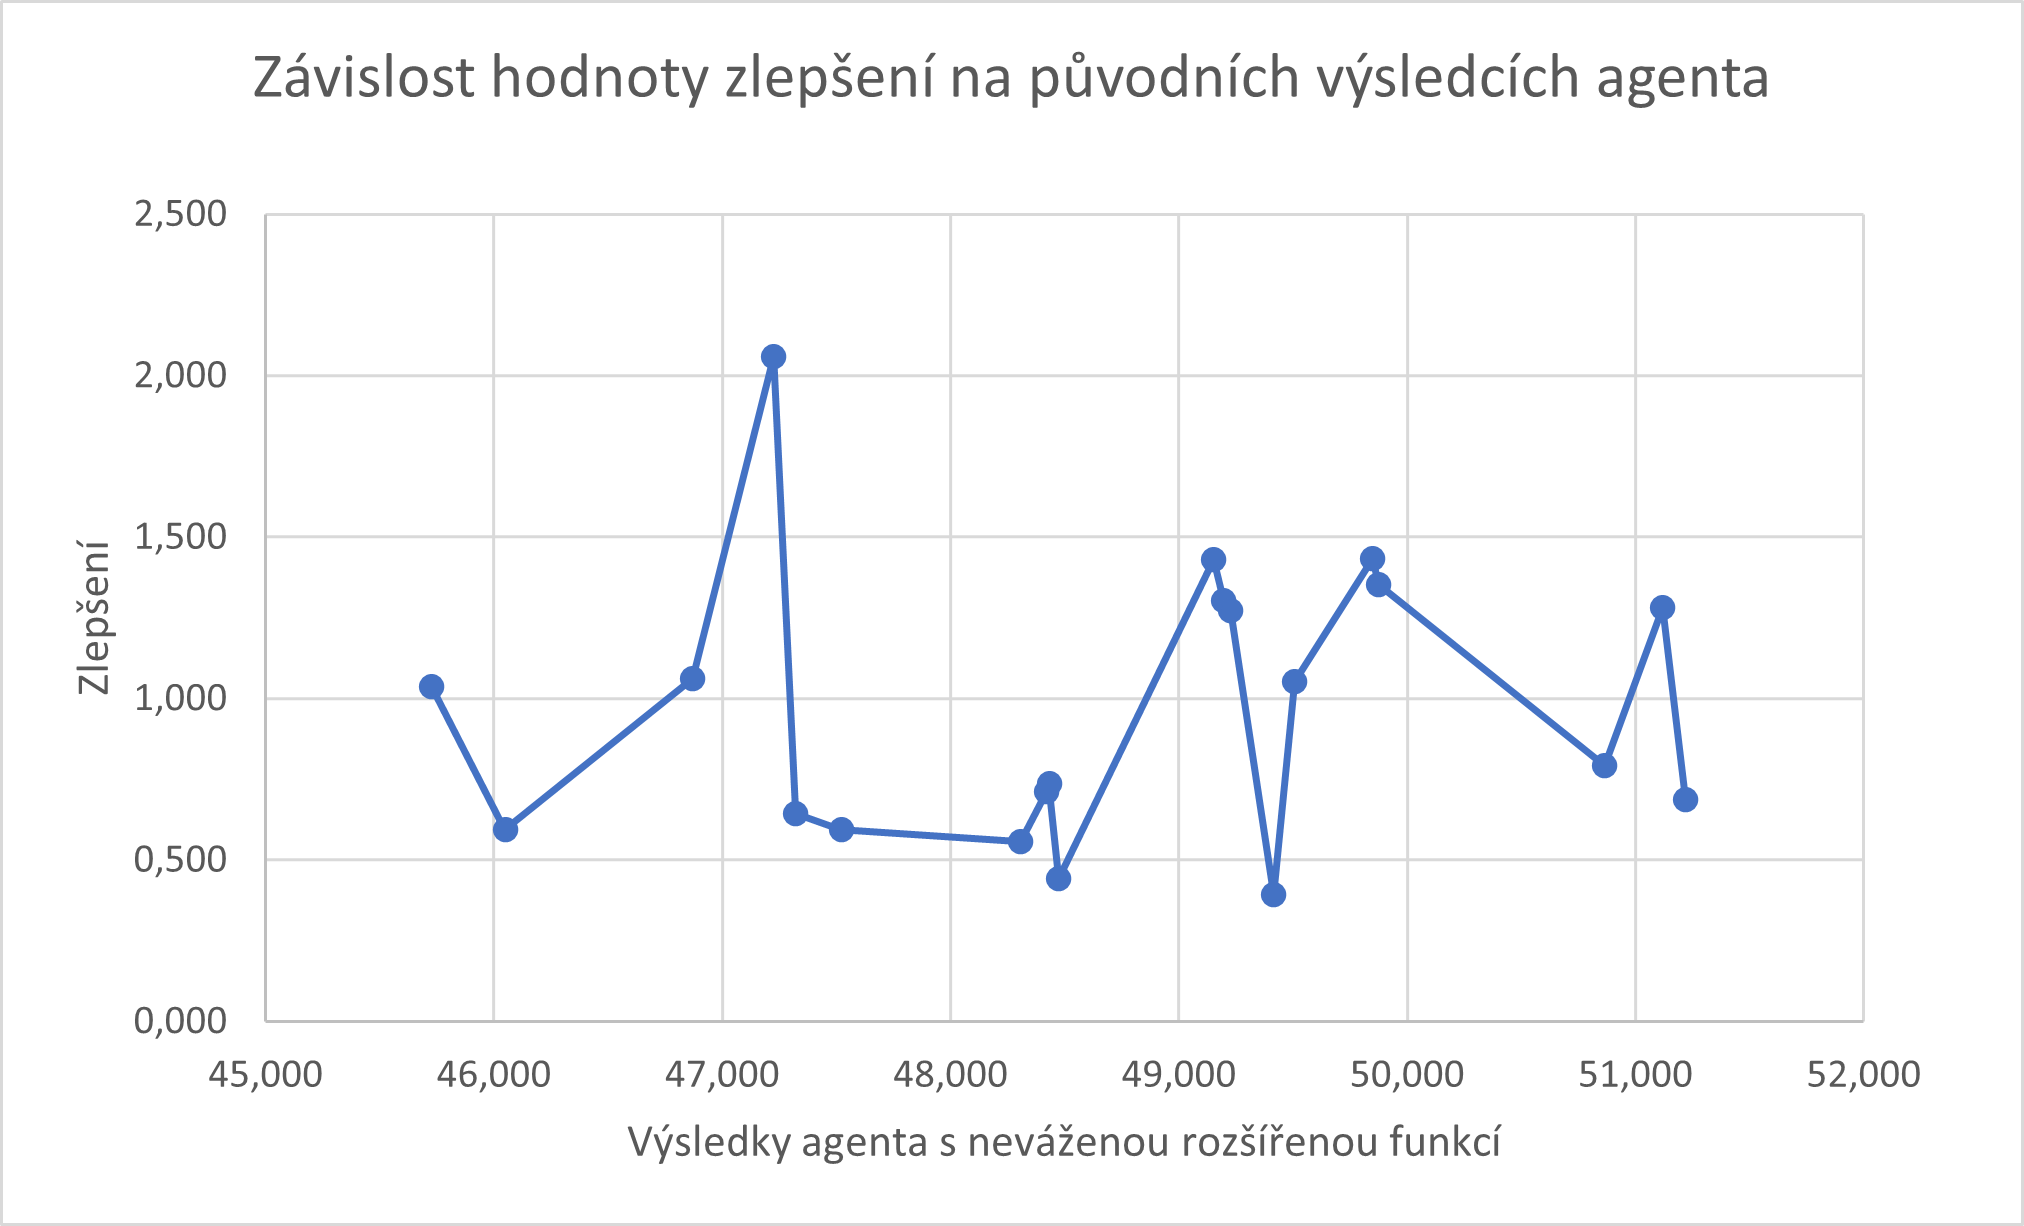
\includegraphics[width=10cm]{cs/obrazky/zavislostZlepseni.png}
    \caption{Graf závislosti}
    \label{fig:zlepseniGraf}
\end{figure}
}

\newcommand{\plotPokus}{
\begin{figure}[H]
\centering
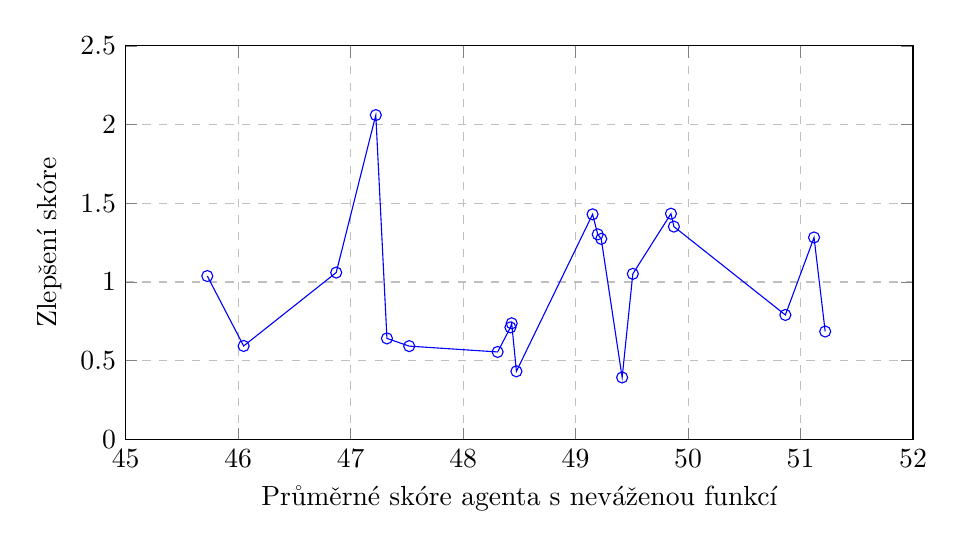
\begin{tikzpicture}
\begin{axis}[
    scale only axis,
    height=5cm,
    width=10cm,
    xlabel={Průměrné skóre agenta s neváženou funkcí},
    ylabel={Zlepšení skóre},
    xmin=45, xmax=52,
    ymin=0, ymax=2.5,
    xtick={45,46,47,48,49,50,51,52},
    ytick={0.0,0.5,1.0,1.5,2.0,2.5},
    xmajorgrids=true,
    ymajorgrids=true,
    grid style=dashed,
]
\addplot[
    color=blue,
    mark=o,
    ]  
    coordinates {
    (45.726,1.038)
    (46.049,0.594)
    (46.872,1.060)
    (47.224,2.060)
    (47.323,0.642)
    (47.521,0.593)
    (48.307,0.556)
    (48.421,0.712)
    (48.432,0.738)
    (48.474,0.433)
    (49.151,1.430)
    (49.197,1.303)
    (49.228,1.274)
    (49.414,0.394)
    (49.509,1.052)
    (49.848,1.434)
    (49.874,1.352)
    (50.865,0.791)
    (51.120,1.283)
    (51.219,0.686)
    };
    
\end{axis}
\end{tikzpicture}
\caption{Graf závislosti zlepšení na původních výsledcích}
\label{graf}
\end{figure}

}
